\subsection{Derivadas em funções de múltiplas variáveis}


\begin{definition} Dada uma função $f: \mathbb{R}^2 \to \mathbb{R}$, definimos as derivadas parciais de $f$ em relação a $x$ e $y$ da seguinte maneira:

\[
f_x(x, y) = \lim_{h \to 0} \dfrac{f(x + h,\; y) - f(x ,y)}{h}
\qquad
f_y(x, y) = \lim_{h \to 0} \dfrac{f(x,\; y + h) - f(x ,y)}{h}
\]

\end{definition}
\textbf{Interpretação geométrica das derivadas parciais}

Seja $z = f(x, y)$ representando uma superfície $S$, e considere o ponto $P(a, b, c)$ onde $c = f(a, b)$. Definimos a curva $C_1$ como a interseção de $S$ com o plano $y = b$, isto é, $C_1: z = f(x, b)$, e a curva $C_2$ como a interseção com o plano $x = a$, ou seja, $C_2: z = f(a, y)$.

As inclinações das retas tangentes às curvas $C_1$ e $C_2$ no ponto $P$ são dadas, respectivamente, por $f_x(a, b)$ e $f_y(a, b)$. Portanto, as derivadas parciais $f_x(a, b)$ e $f_y(a, b)$ podem ser interpretadas geometricamente como as inclinações das retas tangentes em $P(a, b, c)$ aos cortes $C_1$ e $C_2$ da superfície $S$ nos planos $y = b$ e $x = a$.

\begin{figure}[H]
	\centering
	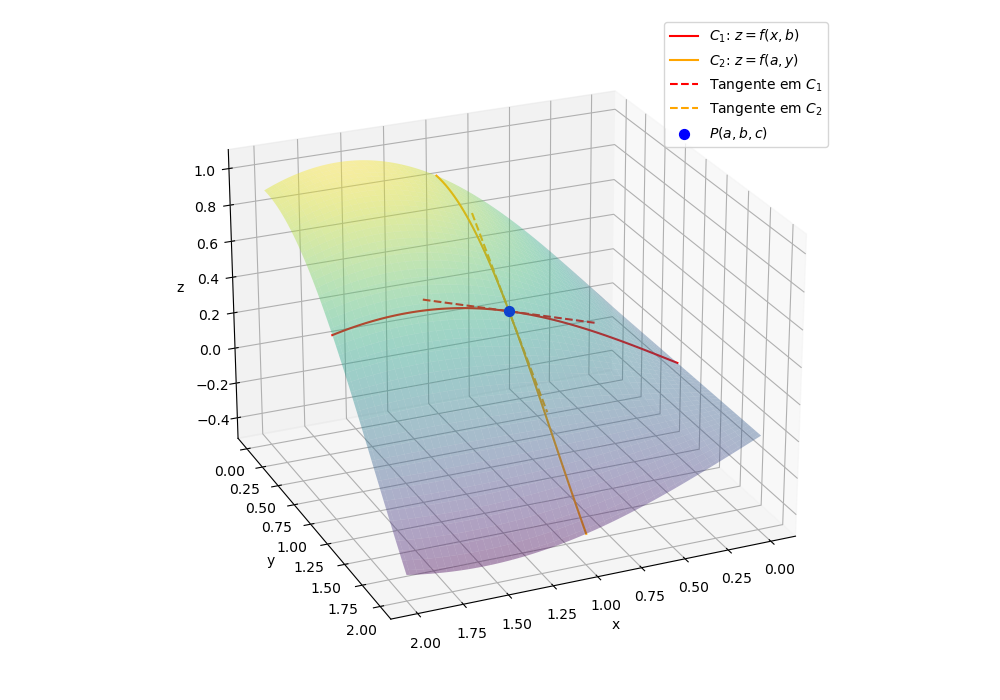
\includegraphics[width=1\linewidth]{pictures/Figure_1.png}
	\caption{Interpretação geométrica das derivadas parciais}
	\label{fig:interpretacao}
\end{figure}

\begin{definition} Dada uma função $f: \mathbb{R}^m \subset \mathbb{R}^n \to \mathbb{R}$, definimos as derivadas parciais de $f$ em relação à i-ésima variável como:

\[
\dfrac{\partial f} {\partial x_i} = \lim_{h \to 0} \dfrac{f(x_1, \dots,x_i + h , \; x_m) - f(x_1 ,\dots, x_m)}{h}
\]

\end{definition}

\begin{definition} Para derivadas parciais de ordem superior:

\[
(f_{x_i})_{x_i} = \dfrac{\partial}{\partial x_i} \left(\dfrac{\partial f} {\partial x_i} \right) = \dfrac{\partial^2f}{\partial (x_i)^2}
\]


\end{definition}

\begin{theorem}
Seja $f$ definida em uma bola aberta $D$ que contenha o ponto $(a, b)$. Se ambas as funções $f_{xy}$ e $f_{yx}$ forem contínuas em $D$, então:

\[
f_{xy}(a, b) = f_{yx}(a, b)
\]

\end{theorem}

